\documentclass{article}
\usepackage{amsmath}
\usepackage{tabularx}
\usepackage{graphicx}

\begin{document}

\title{Section 7.3: Trigonometric Substitution}
\author{Amarnath Patel}
\date{\today}

\maketitle

\section{Introduction}

Trigonometric substitution is a method for solving integrals and differential equations and is often used when the integrand involves the square root of a quadratic polynomial. It is also useful for integrals involving powers of trigonometric functions.

\section{Method}

The method involves substituting a variable with a trigonometric function. There are three main forms of trigonometric substitution:

\begin{itemize}
    \item $x = a \sin(\theta)$, used when the integral contains $\sqrt{a^2 - x^2}$
    \item $x = a \tan(\theta)$, used when the integral contains $\sqrt{a^2 + x^2}$
    \item $x = a \sec(\theta)$, used when the integral contains $\sqrt{x^2 - a^2}$
\end{itemize}

\section{Example}

Let's look at an example. Suppose we want to integrate $\int \sqrt{1 - x^2} \, dx$.

For this integral, we can use the substitution $x = \sin(\theta)$:

\begin{align*}
    \int \sqrt{1 - x^2} \, dx &= \int \sqrt{1 - \sin^2(\theta)} \, d(\sin(\theta)) \\
    &= \int \cos(\theta) \, d(\sin(\theta)) \\
    &= \sin(\theta) + C \\
    &= x + C
\end{align*}

So, $\int \sqrt{1 - x^2} \, dx = x + C$.

The following table lists the common forms of trigonometric substitution:

    \begin{figure}[h]
        \centering
        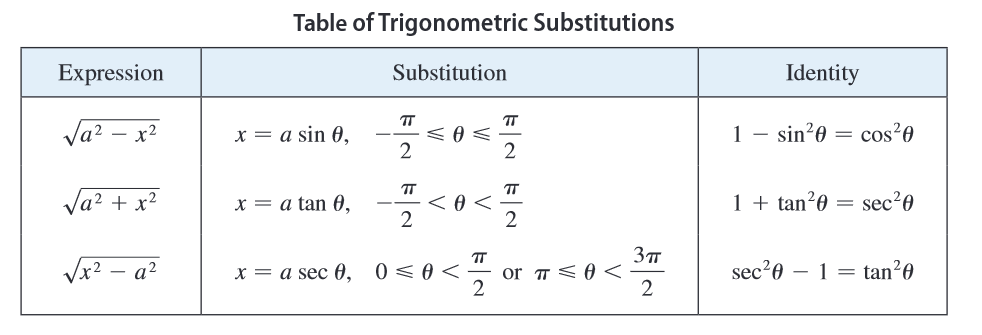
\includegraphics[width=1\textwidth]{../assets/image4.png}
    \end{figure}

    \begin{figure}[h]
        \centering
        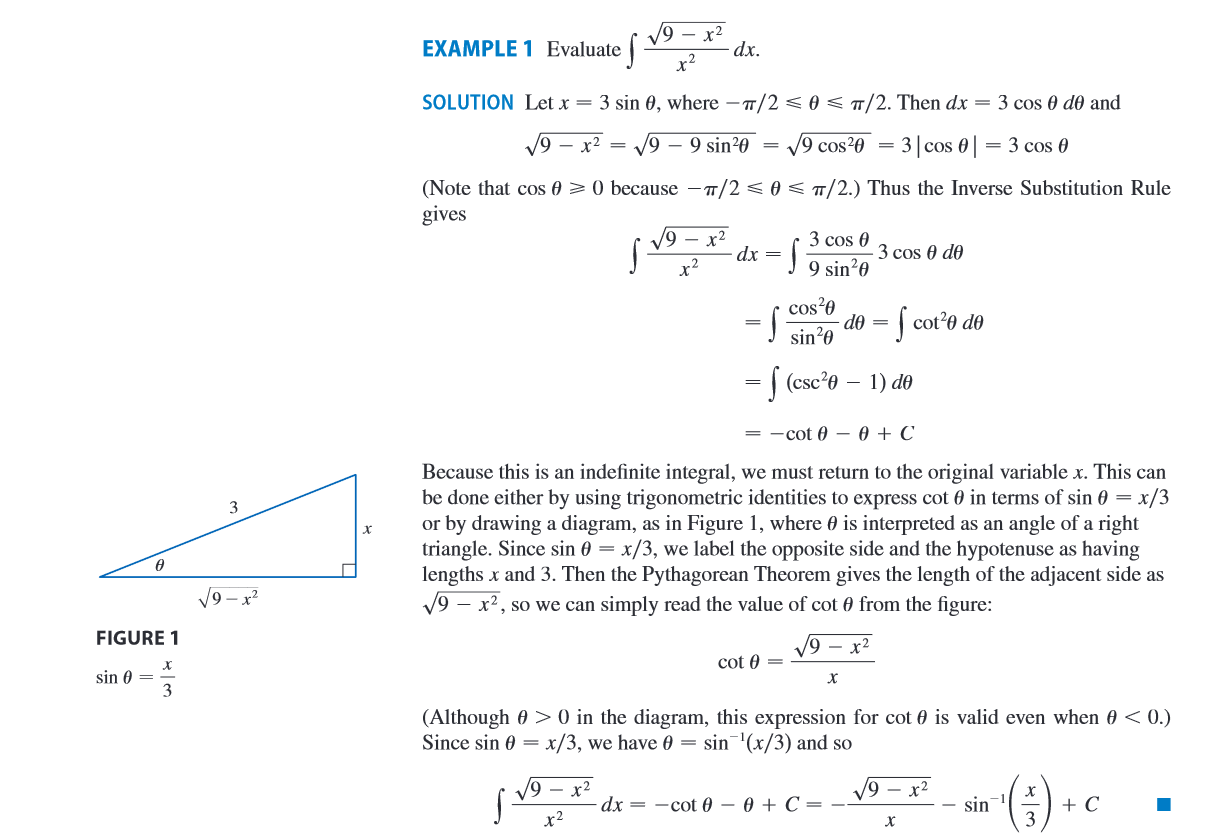
\includegraphics[width=1\textwidth]{../assets/image5.png}
    \end{figure}

    \begin{figure}[h]
        \centering
        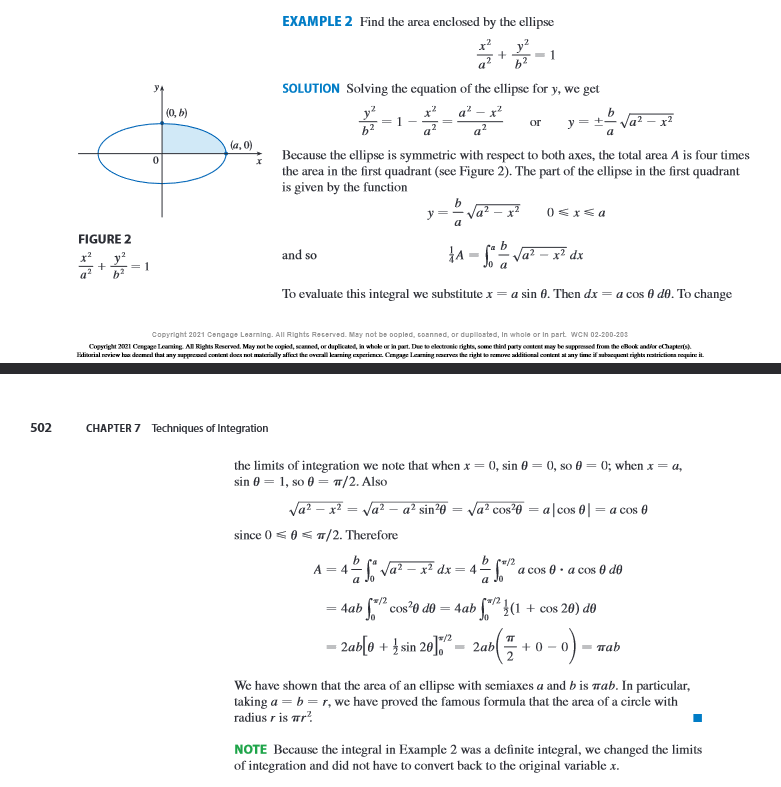
\includegraphics[width=1\textwidth]{../assets/image6.png}
    \end{figure}

    \begin{figure}[h]
        \centering
        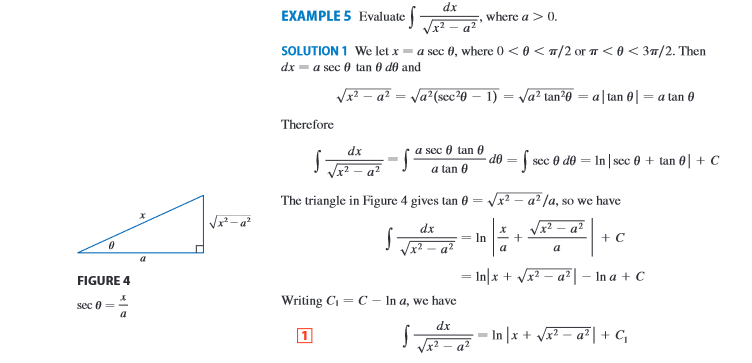
\includegraphics[width=1\textwidth]{../assets/image7.png}
    \end{figure}
\end{document}